%\documentclass[sigconf]{acmart}
\documentclass{article}
\usepackage[margin=1.8in]{geometry}

\usepackage[]{graphicx}
%\usepackage[]{color}
\usepackage{color, colortbl}
\usepackage{subcaption}
\usepackage{listings}
\usepackage{url}
\usepackage{epsfig}

\usepackage{multicol}

\begin{document}

\title{DetGen: Data generation to bridge the "semantic gap" in network intrusion detection}
%Dynamic Traffic Generation with Containerization for Machine Learning}

\maketitle

%\pagebreak

\section*{Contribution page}

\subsection*{Framework}

\paragraph{Controlling traffic influences and detailed label creation}
\begin{itemize}


\item Attention in the setup of lab-capture is most put into attack inclusion and larger network topology, less so into the generation benign traffic, and no attention so far has been spend on controlling the different factors of influence given in Table \ref{Tab:Influence}.

\item[--] We discuss the different influence layers, for well known ones we refer to previous work, for others we demonstrate the effect in experiments. We discuss how we control the influence either through simulation or specific setups

\item[--]

\item Traditional lab-capture setups that consist of a network of virtual or test machines typically capture all traffic in one capture-\textit{channel} at the router without a distinction of different traffic types. Variation in traffic is however introduced at many levels (application type, specific application task, caching/cookies, load/buffering, congestion/loss, etc.), for which information is not  recorded and impossible to recreate through the usual manual or rule-based labelling that is used to identify malicious activity.

\item Through the use of containers, our testbed design facilitates different capture channels and enables us to record  information on these variations for a more complete and granular data capture than traditional setups. Containerised applications isolate task executions more than VM-setups and by capturing traffic directly at each container network interface, we can collect traffic from different applications in different places that would otherwise be merged into the same capture due to being send via the same network interface.

\item We combine this setup with a set of scripted activities with behaviours (FTP-file-transfer, HTTP-website fetch,...) and sub-behaviours (waiting time, transfer fails, ...) that are precisely defined and for which we can extract information-rich labels. This way, we can extract traffic labels containing ground-truth with a very granular resolution on the generating activity.

\item \textbf{Closing the semantic gap}
\begin{itemize}

\item Granular information about the activities and settings generating particular traffic traces enables researchers to match particular traffic structures or model misbehaviour with corresponding computational actions, something that is not possible with current datasets and testbeds. This should help researchers to
better understand the logical small-scale structures in network traffic and understand the effect of different types of traffic on models. 

\item Furthermore, the separation of applications through the use of containers makes our framework modular and enables researchers to quickly swap particular containers to measure the effect of different implementations, or to add different attack types to a setting with \textit{Metasploitable}-containers without having to worry about version-dependent vulnerabilities.
\end{itemize}
\end{itemize}

%\section{Impact factors on traffic micro-structures}
%
%In order to provide extensive ground truth information that describe the traffic we generate, we first must understand what factors have influence on the traffic generation process. \textcolor{red}{How do we verify that this list is more or less complete?}
%
%\paragraph{Application layer protocols} 
%Without doubt the biggest impact on the captured traffic micro-structures is the choice or combination of the application layer protocols. Protocols such as HTTP/TLS perform vastly different tasks than protocols such as Peer-2-Peer or SMB, and thus perform different handshakes, experience different waiting times, transfer data in different intervals, or trigger different additional connections. 
% 
%\paragraph{Performed task and application}
%The conducted computational task ultimately drives the communication between computers, and thus hugely influences characteristics such as the direction of data transfer, the duration and packet rate, packet sizes as well as the number of connections and performed protocol handshakes to conclude the task. Furthermore, the application used for the task has a significant influence on the generated traffic, as shown for different browser choices by Yen et al. \cite{yen2009browser} or for general application behaviour fingerprinting \cite{stober2013you}. 
%
%\paragraph{Transferred data} 
%The amount of transferred data obviously influences the overall packet numbers. Furthermore, the content of the data can potentially impact packet rates and sizes, such as shown by Biernacki \cite{biernacki2017analysis} for streaming services.
%
%\paragraph{Caching/Repetition effects}
%Tools like cookies, website caching, DNS caching, known hosts in SSH, etc. can cause to parts of a communication being skipped and lead to differences in the captured traffic between initial and subsequent connections.
%
%
%\paragraph{Application layer implementations}
%Different implementations for TLS, HTTP, etc. can yield different computational performance and can perform handshakes in slightly different ways. Furthermore, things like multiplexing channel prioritisation can have tremendous impact on the IAT times and the overall duration of the transfer, as shown in a study by Marx et al.  \cite{marx2020same} for the QUIC/HTTP3 protocol.
%
%\paragraph{Networking stack load}
%TCP or IP queue filling due to other applications generating traffic can alter IATs of the traffic trace and affect available bandwidths. \textcolor{red}{We should perform an experiment using iperf, once with TCP and once with UDP to quantify the effect}.
%
%\paragraph{Host level load}
%In a similar manner, other applications exhibiting significant computational load (CPU, memory, I/O) on the host machine can affect the processing speed of incoming and outgoing traffic, which can again alter IATs and the  overall duration of a connection. \textcolor{red}{We should perform an experiment using \textit{stress} to quantify the effect}.
%
%\paragraph{LAN and WAN congestion}
%Low available bandwith, long RTTs, or packet loss can have a significant effect on TCP congestion control mechanisms, which in turn influence frame-sizes, IATs, window sizes, and the overall temporal characteristic of the sequence. \textcolor{red}{do we need to verify this? Seems very clear}
%
%\vspace{0.3cm}
%Other factors we are currently not considering:
%
%\paragraph{User and scheduled activities}
%The frequency with which a user or an application performs tasks governs the larger-scale temporal characteristic of a traffic capture. Since we are focusing on the traffic micro-structures here, we currently omit this impact factor from our analysis. 
%
%\paragraph{TCP congestion management implementation}
%Different versions of the TCP congestion manager exist on Windows and Linux such as TCP Reno/Tahoe, which can have minor influence on the traffic, as shown by Grieco et al. \cite{grieco2004performance}. Existing implementations on a machine stay mostly constant, which is why we also omit this variable at the moment.
% Implementations within a machine should stay constant.
%
%\paragraph{Network configurations}
%Network settings such as the MTU or the enabling of TCP Segment Reassembly Offloading have effects on the captured packet sizes, but like TCP implementations stay mostly constant for a host. 
%
%\textcolor{red}{....}

%\begin{table}
%\begin{tabular}{p{2.5cm}|p{3cm}|p{8cm}}
%Influence& Level & Description \\ \hline \hline
%
%Higher level influence&
%User and scheduled activities&
%How often the user accesses which services, or how often and when a system updates information\\ \hline 
%
%
%Major influence&
%Application used&
%This governs what application layer protocols are used, how often and in what order. As an example, despite doing the same thing, Chrome and Firefox send HTTP-Get requests in different orders and open different numbers of connection sockets\\ \hline
%
%Minor influence&
%Transferred data&
%The size of the transferred data influences overall packet numbers, and potentially the packet rates and sizes (for example streaming high-quality vs low quality), as can the data type.\\ \hline
%
%Major influence&
%Application memory&
%Applications often cache content, credentials, DNS records or cookies from previously contacted hosts\\ \hline
%
%Biggest influence& 
%Application layer protocols &
%Different application layer protocols obviously follow different communication protocols, send data differently, and trigger additional connections in different ways\\ \hline
%
%
%Minor/major influence&
%Application layer implementations&
%Different implementations for TLS, HTTP, etc. can have differing performance, which influences packet IATs and potentially TCP buffering. They can furthermore often differ in minor ways such as different handshakes etc., and occasionally in major ways such as HTTP multiplexing implementations which differ wildly in the channel prioritisation\\ \hline
%
%
%Potential minor influence& 
%TCP implementation&
%There are different implementations of TCP on Windows and Linux such as TCP Reno/Tahoe, which can have minor influence on the traffic but they should stay the same on a machine\\ \hline
%
%Minor influence&
%Network interface load&
%TCP buffer filling due to other programms communicating (both in forward and receiving direction). Potentially other buffers or similar in the networking stack, and therefore the overall bandwidth available\\ \hline
%
%Minor influence&
%Host level load& \\ \hline
%
%Major influence&
%LAN and WAN & Congestion, low bandwith, or loss can have a significant effect on TCP (and others like QUIC) congestion control mechanisms, which in turn influence frame-sizes, IATs, window sizes, ....
% \\ \hline
%
%Minor influence&
%Network configuration&MTU, MTU path discovery, and TCP Segment Reassembly Offloading \\ \hline
%\end{tabular}
%\caption{Influence factors}\label{Tab:Influence}
%\end{table}

\begin{figure}
\centering
\begin{subfigure}[b]{0.46\textwidth}
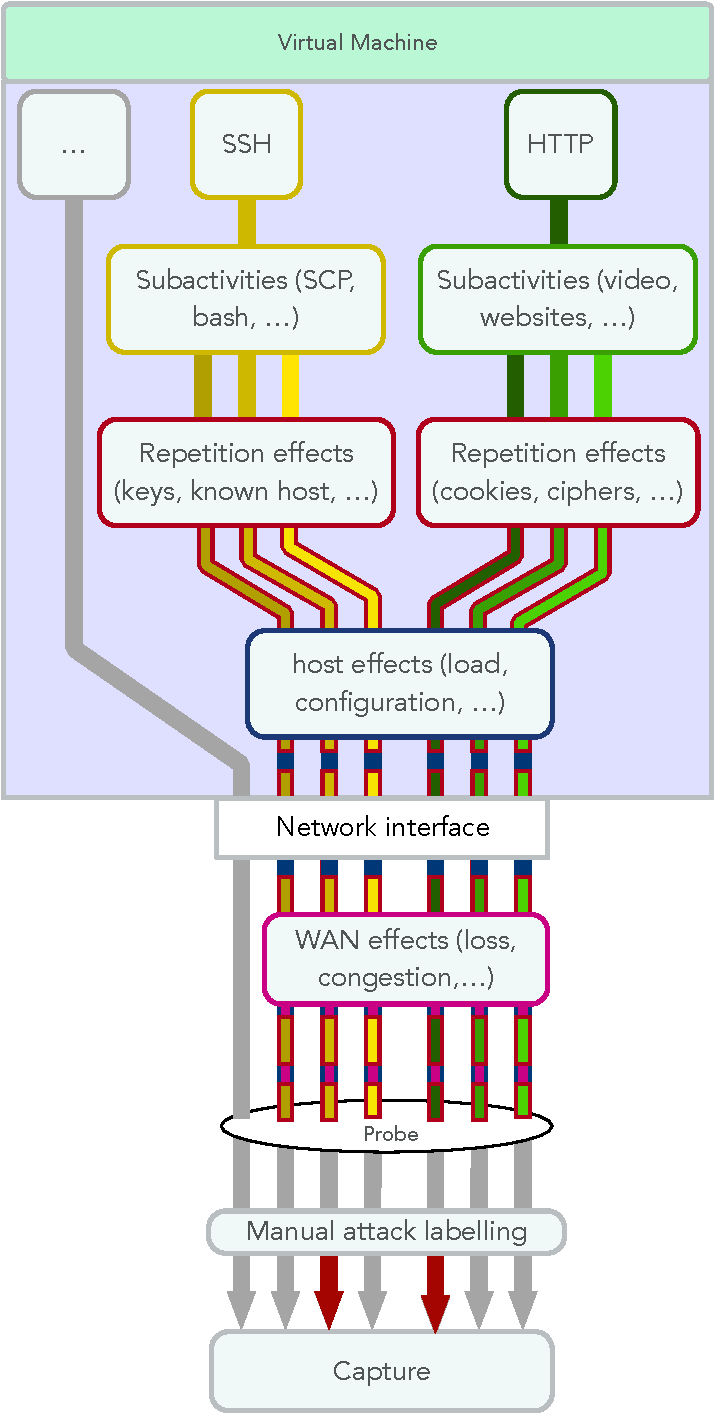
\includegraphics[width=\textwidth]{images/VM_capture.pdf}
\caption{Traditional capture setup}
\end{subfigure}

\begin{subfigure}[b]{0.8\textwidth}
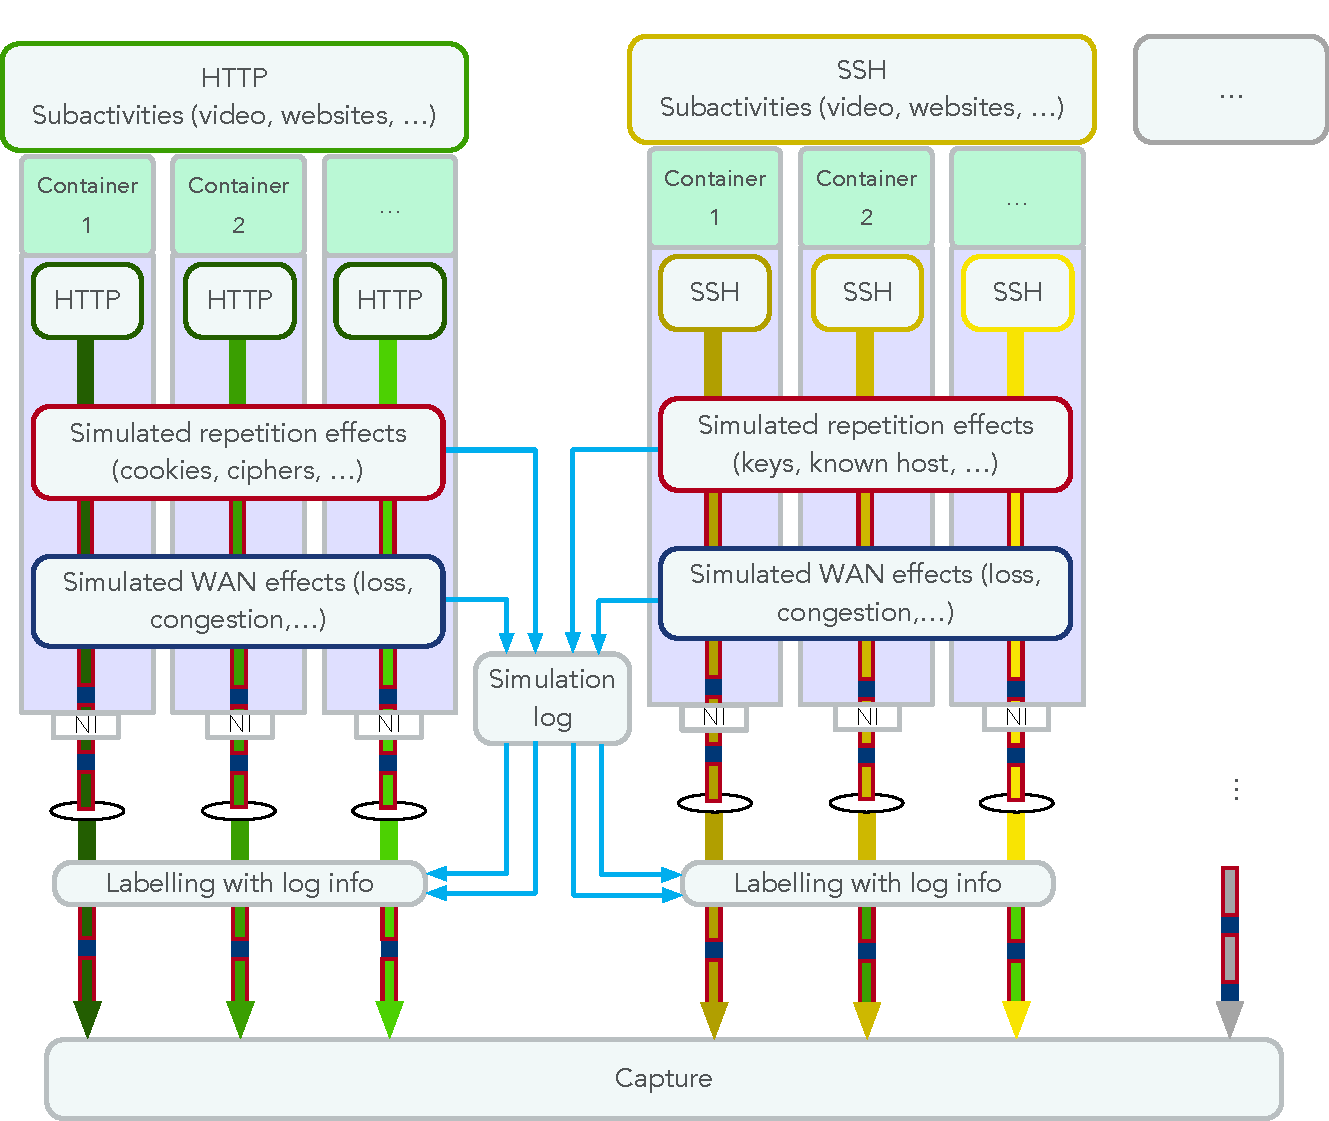
\includegraphics[width=\textwidth]{images/Docker_capture.pdf}
\caption{Our container-based capture setup}
\end{subfigure}
\end{figure}

\paragraph{Reproducibility}

%%As computational work becomes more and more integral to many aspects of scientific research, computational reproducibility has become an issue of increasing importance to computer systems researchers and domain scientists alike.

Several factors in our design contribute to making the data and corresponding network experiments \textcolor{red}{particularly} reproducible:

\begin{itemize}

\item Docker containers by design operate platform-independent without the need for muddled dependencies, and the separation of running containers from container images in contrast to VMs guarantees repeatable tasks without "code rot".

\item We introduce adjustable degrees of input (files, passwords,...) and traffic (congestion, network fails) randomisation for our scenarios, with labels describing the particular setting being extracted. This way, similar scenarios and settings can be easily recreated.

\item Intrusion detection systems in the form of firewalls or \textcolor{red}{...} can be included directly in the framework as containers to enable other researchers to verify the achieved results.

\end{itemize}


%Ground truth labels on granular activities 

%Isolated process in container, no additional events. Easy to separate even when containers attached to same network interface & background events (system activitiy, artifacts from earlier activity, ...), overlaying activities hard to separate & No knowledge about conducted activity & Technically possible, no attempts yet \\ \hline

%Reproducability & Container state the same after repeated launches, isolation means that other task have little effect on, plattform independence  & To a lesser degree, simultaneously conducted activity can affect each other & - & Depends \\ \hline


\subsection*{Analysis}

Details on our use-cases and framework analysis

\pagebreak


\section{Introduction}



%Data-driven traffic analysis and attack detection is a centrepiece of network intrusion detection research, as well as many other fields \textcolor{red}{citations}. 
In this work, we introduce a new design paradigm for traffic generation testbeds that addresses the \textit{semantic gap} in network intrusion detection by closely controlling different factors that influence generated network traffic and providing cross-linkage information between captured traffic and these factors. Our design relies on a composition of containers to enable capturing traffic directly programs that run in an isolated and reproducible manner. Rather than simulating the large-scale behaviour of users in a realistic way, we aim to generate small-scale traffic scenarios that contain true interactions between software components in a realistic way to enable researchers a better understanding of particular traffic events. 

Data-driven traffic analysis and attack detection is a centrepiece of network intrusion detection research, and the idea of training systems on large amounts of network traffic to develop a generalised notion of bad and benign behaviour appears  like the solution to cyber-threats and has received \textit{tremendous} attention in the academic literature. However, operational deployment is dominated by systems relying on less \textcolor{red}{generalised} attack signatures. Already in 2010 Paxson and Sommer \cite{sommer2010outside} have identified a number of \textcolor{red}{issues} that are summarised as an overall lack of connection between the nature of intrusion detection data and the applied data-driven detection systems, something the authors call the `semantic gap'. These findings have since then been confirmed by other authors such as Harang \cite{harang2014bridging} in 2014 or by Liu et al. in 2019 \cite{liu2019machine}.

Among others, these issues include (1) fundamental difficulties for conducting sound evaluation of detection models \textcolor{red}{and a (2) lacking perspective of a network operator that handles alerts,} that result in a (3) semantic gap between the development of detection models and the structural and operational nature of network traffic and intrusion detection. 

\textcolor{red}{Data-centric} breakthroughs in other fields have not been achieved solely by more complex and computationally more powerful ML-methods, but have been equally reliant on a precise understanding of the data and corresponding datasets that provide researchers with richer information and enable them to analyse weak points and model failures. As an example, results in \textit{automatic speech recognition (ARS)} were not achieved by immediately training models on simply large annotated datasets. Initial models were reliant on highly sanitised and structured speech snippets in order to isolate low-level structures such as phonemes or time-warping. Lately, datasets that contain labelled specialised speech characteristics with varying intensity enable researchers to better understand ASR weak points such as emotional speech (RAVDESS), accents (Speech Accent Archive), or background noise (Urban Sound Dataset).

%As an example, results in  were not achieved solely by training models on large annotated datasets, but have been reliant on specialised datasets that highlight and label speech structures such as emotions (RAVDESS dataset), noise, or accents 

%between results and their operational interpretation.

In a similar fashion, several approaches to enhance the way information is collected and presented have been successful in closing semantic gaps between data and detection systems in other areas of information security. Virtual machine introspection monitors and analyses the runtime state of a system-level VM to improve the understanding of virtual machine-based intrusion detection and forensic memory analysis \cite{dolan2011virtuoso}. The inclusion of threat reports to create behavioral feature labels enriches the way executables are described to enhance malware modelling and detection \cite{smith2020mind}.

However, such efforts have not been made in network intrusion detection yet, with the current \textcolor{red}{benchmark} datasets paying more attention to the inclusion of a wide variety of attacks rather than the close control and detailed documentation of the generated traffic structures. This has so far lead to researchers predominantly applying of a number of ML-models directly to \textcolor{red}{general} traffic datasets in the hope of edging out competitors without analysing what traffic causes the model to fail and how design choices could prevent that.


%By moving from virtual machines to containers, we enable the scalable, modular, and dynamic creation of network traffic datasets. Since containers can be arranged in complex settings with a few commands, it is a lot easier with containers to script a variety of network activities thus increase the heterogeneity and realism of the generated data.

 
%We propose a novel design paradigm that makes generation of network traffic and corresponding attacks significantly more flexible and offers a \textcolor{red}{new level} of insight and reproducibility for traffic micro-structures through the use of containerisation. 
This work provides the following contributions:

\begin{enumerate}
\item We propose a novel design paradigm for generating reproducible small-scale traffic structures with ground-truth labels that contain extensive information about the computational interactions behind it. 
\item We present a novel and extensible network traffic generation framework called \textit{DetGen} that implements our design paradigms to improve several shortcomings of current data generation frameworks for NIDS evaluation.
\item We perform a number of experiments to demonstrate the fidelity to realism of the generated data.
\item We present a number of use-cases to demonstrate how the design of our framework can boost evaluation and enhance understanding of ML-based network intrusion detection systems to close the semantic gap described by Sommer and Paxson \cite{sommer2010outside}.
%\begin{enumerate}
%\item Ground truth labels documenting every conducted activities
%\item Increased structural realism of the data on a packet-level
%\item Tunable topology, traffic composition, and attack types
%\item Capture of program logs and system calls for data fusion methods
\end{enumerate}

This framework is openly accessible for researchers and allows for straightforward customization.

%Realistic network traffic datasets allow engineers to build a better understanding of existing structures, motivate design choices from actual needs, and prove that proposed new systems can indeed work in practice. \textcolor{red}{something to emphasise that packet traffic is important.}

%Unfortunately, privacy and security concerns discourage network administrators to release rich and realistic datasets for the public,  leading to publicly available real-world datasets being the exception and missing informative features such as captured packets or consistent IP-addresses. As a result, researchers are predominantly relying on synthetically generated data, which is currently either captured using scripted activities in a virtual or lab-environment, or generated using trained generative models of real-world traffic.

%Existing network intrusion detection datasets are however collected in a static manner, unable to be modified, updated, or reproduced, \textcolor{red}{citation} and therefore can neither adapt to novel attacks or traffic evolutions, nor give researchers the flexibility to focus on particular traffic types. Furthermore, the current capture setups provide no insight in the data generation process, and it is mostly impossible to match events on the packet-level with conducted activities due to the capture setup. 
%Existing testbeds and traffic generation frameworks are successful at emulating large-scale traffic characteristics \textcolor{red}{citations}, but fail to provide the necessary detail and realism for intrusion detection on a packet-level. 

%This proves to be a serious defect as the ecosystem of intrusions is continually evolving.
%Furthermore, it prohibits a more detailed analysis of specific areas of network traffic due to the available data only being a fraction of the original dataset. To combat this, new datasets must be periodically built from scratch.


%Furthermore, VM-based traffic simulation frameworks provide little insight into the ...


%Allowing researchers to create datasets dynamically to circumvent these issues would be extremely beneficial. 

%Furthermore, each Docker container is highly specialized in its purpose, generating traffic related to only a single application process. Therefore, by scripting a variety of Docker-based \emph{scenarios} that simulate benign or malicious behaviours and collecting the resultant traffic, we can build a dataset with perfect ground truth, something that has so far not been possible for network traffic. 



 
%\item We define four new requirements a network intrusion dataset should fulfil in order to be suitable to train machine-learning based intrusion detection methods. 
 %\item how to build new modules that can be added to the existing framework, and how this procedure enables data generation that is more suitable for data-driven methods than currently available datasets.
% \item We perform a number of experiments to demonstrate the fidelity to realism of the generated data.
%\item We present a number of use-cases to demonstrate how the design of our framework can boost performance for ML-based network intrusion detection systems, in particular for false-positive analysis and effective model training.
%\end{enumerate}

%\subsection{Contributions}

%\subsubsection{Main contributions}


%
%\begin{enumerate}
%\item Fidelity to real traffic
%\begin{itemize}
%	\item Real traffic, consistent (not invalid after Cordero et al.)
%	\item Structural richness on packet level (in contrast to )
%		Induced due to the different levels at which traffic variation is introduced
%%	\item Temporal activity levels? (actually not something we improve)
%%			We can look at test for realism of distributions (IP discovery, etc)
%\end{itemize}
%\item Ground truth labels through containerisation
%\begin{itemize}
%	\item Ground truth for attack behaviour, able to label 100\% of the generated events to specific activities
%	\item Labels for different types of behaviour, reproducable
%		useful for evaluation of model failures, what kind of behaviours cause failure
%			applies to a large range of models
%		also useful for evaluation of privacy infiltration methods, more niche
%	\item Ground truth for label matching between traffic and program logs/sys logs
%		useful for models that try to correlate events for detection
%			this is more niche, but potentially because of the lack of data
%\end{itemize}
%\item Extensive capture
%\begin{itemize}
%	\item Packet availability
%	\item Syslogs and for multiple scenarios program logs
%	\item Potentially host logs? Depends if we want to cater to cloud computing applicability
%\end{itemize}
%\item Better for ML-based methods
%\begin{itemize}
%	\item Flexibility 
%		"The models should allow researchers to generate different classes of data, such as augmenting the amount of data representing sparse events, or choose different topology"
%	\item Automisation of variable datasets through randomisation, automatically create structurally different datasets, but faithful to realism
%		Especially novel in terms of network topologies, should emphasise this in use-cases
%	\item Structural richness 
%			allows for learning deeper and more generalisable knowledge in models, less prone to overfitting
%	\item Scalability
%		"Train on as much data as necessary"
%\end{itemize}
%
%\end{enumerate}





\subsection{Outline}

%The remainder of the paper is organized as follows. Section \ref{Sec:background} discusses existing NIDS datasets and the problems that arise during their usage as well as background information about network traffic data formats and virtualization methods. The section concludes with a set of requirements we propose to improve the training and evaluation of machine-learning-based methods. Section \ref{Sec:Design} describes the general design of our framework, and how it improves on the discussed problems in existing datasets. We also discuss a specific example in detail. Section \ref{Sec:Experiments} discusses several experiments to validate the improvements and utility our framework provides. 
%Section \ref{Sec:Conclusion} concludes the results and discusses limitations of our work and directions for future work.

Outline of the coming sections.

\dots \dots

\dots \dots

\dots \dots




\section{Background}

\subsection{Misuse and machine learning}


Network intrusion detection is the field of detecting intrusions in a network by analysing captured traffic traces exchanged between computers in the network. Most commonly used are misuse detection systems identify known signatures of bad behaviour in traffic such as malicious packet payloads or rule-based patterns concerning port usage and/or packet sequences. Although very efficient, these methods are reliant on precise details on known attacks in the form of signature databases. Significant efforts have been invested in developing machine-learning based methods that are trained on large amounts of traffic to develop a more generalisable distinction between benign and malicious behaviour to remove the need of attack signatures and enable the detection of zero-day attacks.


\subsection{Existing problems}

Machine-learning based network intrusion detection has been subject to extensive criticism due to being unable to deliver sufficient detection rates at an acceptable false-positive rate in actual deployment. A number of causes for these failings have been identified particularly for network-based methods by Sommer and Paxson \cite{sommer2010outside} in 2010, which have been supported and partly extended by Harang \cite{harang2014bridging} in 2014 or by Liu et al. in 2019 \cite{liu2019machine}:


\paragraph{Semantic gap between between results and their operational interpretation}

Arguably the biggest concern expressed by Sommer and Paxson is that methods lack a deep semantic insight into a system's capabilities and limitations and are instead treated as black boxes. The authors here draw comparisons to other areas of machine learning such as character recognition where the precise understanding of the data structure and how existing systems process it have lead to breakthroughs such as the convolutional layers that process the data in a more adequate way. In network intrusion detection, different methods are thrown at existing data without thorough analysis where the system performs well and where it fails or breaks, and what the reasons for this are. The authors recommend to researchers to narrow the scope to more specific applications and closely examine what types of traffic trigger which responses by the system in order to develop a better understanding of where and how future systems can be designed to better suit this particular type of data and application. 


%\begin{itemize}
%%\item " To address them, we deem it crucial for any effective deployment to acquire deep, semanticinsightintoa system’s capabilities and limitations, rather than treatingthe system as a black box as unfortunately often seen."
%
%\item understanding the system’s semantic properties—the operationally relevantactivity that it can detect, as wellas theblind spotsevery system will necessarily have
%
%\item If we could give onlyonerecommendation on how toimprove the state of anomaly detection research, it would be:Understand what the system is doing
%
%\item an area whereinsightmatters much more than just numericalresults
%
%\item What can it detect, and why? What can itnot detect, and why not? How reliably does it operate?Where does it break?
%
%\end{itemize}


\paragraph{Fundamental difficulties for conducting sound evaluation}

The semantic gap stems in part from persistent difficulties for researchers to evaluate their system thoroughly and in a comparable and reproducible manner due to a lack of appropriate public datasets. Privacy and security concerns discourage network administrators to release rich and realistic datasets for the public,  leading to publicly available real-world datasets being the exception and missing informative features such as captured packets or consistent IP-addresses. This forces researchers to generate synthetic datasets using small virtual networks, and restricts the diversity and coverage of traffic researchers are able to examine.

Furthermore, the labelling process is significantly more difficult in network intrusion detection than in other domains with easier interpretable data. Often, only traffic directly involved in an attack is labelled manually, with all other traffic receiving the same `Benign' label. This lack of informative labels impedes researchers abilities to analyse different types of traffic and thus understand the properties of their system.

The lack of benchmark datasets often forces researchers to assemble their own data, which is mostly done in a non-reproducible way, leading to unverifiable detection rates and incomparable results.

%network traffic appropriately is significantly more difficult 

%As a result, researchers are predominantly relying on synthetically generated data, which is currently either captured using scripted activities in a virtual or lab-environment, or generated using trained generative models of real-world traffic


%\begin{itemize}
%\item understanding the system’s semantic properties—the operationally relevantactivity that it can detect, as wellas theblind spotsevery system will necessarily have

%\item reproducibility 

%\end{itemize}

%\paragraph{Lacking perspective of a network operator}

%Network intrusion detection is not just a task of classifying traffic, but is a tool in securing a network during its operation. For that, it needs to support the network operator in understanding the flagged activity and enabling a quick assessment of its impact in the context of the network environment. Again, current datasets already provide little insight into the context of traffic events or domain knowledge, making it hard for researchers to develop a model that can provide this context, leading to simple numerical evaluations on static data that neglect this perspective.

%\begin{itemize}
%\item the nex tstep then needs to interpret the results from an operator’spoint of view—“What does it mean?

%\item understanding how thefeaturesthe anomaly detectionsystem operates on relate to the semantics of the networkenvironmen

%\item In addition to correctlyidentifyingattacks,an anomaly detection system also needs to support theoperator in understanding the activity and enabling a quickassessment of its impact
%\end{itemize}

\vspace{0.2cm}
Other problems identified by Sommer and Paxson include the diversity of network traffic, the high cost of errors, and lacking computational speed or detection systems.

\section{Goals and motivation}

Our goal in building \textit{DetGen} is to provide a framework that generates information-rich and reproducible network traffic to help researchers understand traffic micro-structures and how they impact the performance of detection models in order to close the existing semantic gap and provide reproducible and verifiable network experiments. We focus on traffic micro-structures because even though many NID systems operate on this level, there exists little comprehensive research on general traffic behaviour\footnote{Exceptions being on models for application fingerprinting} on the packet level, whereas longterm or network-wide traffic structures is far better understood \textcolor{red}{should I insert citations here? \cite{willinger1998self}}.

We position our framework against NID data generation setups, such as those used in the CICIDS-17 or the UNSW-15 datasets \cite{moustafa2015unsw,sharafaldin2018towards}. These setups are regularly used to ....

%\textcolor{red}{explain why focus on micro-structures and not larger structures}
%We set out the following priorities:


%enables researchers to conduct reproducible and informative network experiments in  

%\subsection*{Primary goals}



\paragraph{Rich ground truth information} Attention in the setup of typical lab-capture environments is put primarily into attack diversity and realistic network topologies and to some extent to the overall generation mechanisms of benign traffic. No attention so far has been spend on controlling and monitoring the different factors, described in Section \ref{Sec:Impactfactors}, that influence how traffic, benign and malicious, is shaped in the generation process. 

Our framework should above all produce ground truth information about the underlying activities of all captured traffic. This information should not only distinguish between benign and malicious activity, but give detailed information about the conducted computational activities. Furthermore, our framework should control and record all necessary factors that impact and shape the generated traffic such as network congestion or transmission failures to better facilitate understanding the effect of different traffic structures and particular phenomena on a detection system.

%\paragraph{Functional realism} Researchers should have the ability to embed their NIDS into our framework in order to enable real-time detection experiments as well as corresponding operator decision-making.

\paragraph{Reproducibility} The scientific method dictates that experiments must be reproduced  before  they  are  considered  valid. Typical setups generate and collect data in a one-shot manner, without control over various quasi-random influences that affect the capture process. Furthermore, the particular setups are often complex and difficult to recreate. This makes is difficult for researchers to reproduce datasets and corresponding network experiments, especially when proprietary customized datasets are used. 

Our framework should be able to precisely reproduce any generated traffic events and corresponding network experiments in order to facilitate verifiable and comparable research. Data should be produced in a controllable manner, with typically random impacts on traffic capture such as transferred data or host load being randomised and monitored in a controlled fashion to enable precise reproduction. We aim at avoiding complicated setups and plattform dependencies in the generation process. 

\paragraph{Traffic realism on a packet level} As described in the first paragraph, attack-focused synthetic intrusion detection data setups so far have paid little attention to the realism of traffic on a packet-level, and exhibit far less event diversity than real-world captures due to the neglect of \textcolor{red}{request diversity} and the shielding from real-world factors such as excessive host load or network failures. We provide examples of this in Section \textcolor{red}{insert Section number}.

The DetGen framework should address these issues and produce traffic that exhibits realistic levels of structural trafficdiversity and rare events. This is a necessary condition to provide a corresponding evaluation of NIDS systems with a plausible degree of scientific insight and relevance. %Internet traffic overall is hard to model, which is why we narrow the scope to the generation of small-scale traffic scenarios that contain true interactions between software components in a realistic way. Furthermore, our framework should enable the inclusion of large-scale network activity profiles to leverage existing research in this area.

%\subsection*{Secondary goals}

%\paragraph{Flexibility} It should be easy to tune the composition of the generated. Similarly, it should be easy to create an experiment with any topology.

%\paragraph{Attack diversity} Intrusion detection models are dependent on attack data that represent specific attacks. The platform should therefore enable the execution or addition of a wide variety of attacks.



\begin{table}
\centering
\begin{tabular}{p{3cm}|p{3cm}|p{3cm}|p{2cm}|p{2cm}}
Contribution&How containers enable it& VM-based & Real traffic capture &Other framework  \\ \hline

Ground truth labels on granular activities & Isolated process in container, no additional events. Easy to separate even when containers attached to same network interface & background events (system activitiy, artifacts from earlier activity, ...), overlaying activities hard to separate & No knowledge about conducted activity & Technically possible, no attempts yet \\ \hline

Reproducability & Container state the same after repeated launches, isolation means that other task have little effect on, plattform independence  & To a lesser degree, simultaneously conducted activity can affect each other & - & Depends \\ \hline


%Flexibility to regenerate customized datasets & Launching a network of containers is easy, modularity allows finer control of fine-grain activity  & Difficult to regenerate data as set-up and launching of VM is less straightforward, might be addressed with MiniMega & No & Yes \\ \hline

Easy to update, include new attacks & 
Attack/victim containers remove dependence on vulnerabilities, can be hooked to existing scenarios with shared resources & Since attacks happen on the VM, it is very hard to compose a VM with enough vulnerabilities to include many attacks & - & Some work has been done to "replay" or artificially inject attacks  \\ \hline


%Fidelity to real traffic heterogeneity, structural richness & Not a lot except that scripting and randomising different scenarios is slightly easier  & Potentially, but little attention has been paid & Yes & Not on a packet level yet \\ \hline \hline


Data on attacks on container isolation & In need of existing scenarios for background data & No & No & No \\ \hline
\end{tabular}
\caption{Contributions compared to existing solutions}\label{Tab:Contributions}
\end{table}

%\vspace{0.3cm}

%Table \ref{Tab:Contributions} compares how well existing methods are realising these goals compared to our framework.


\subsection*{Motivational use-cases}% \textcolor{red}{(or Use-cases?)}}

While there are many potential use-cases that can benefit from a system like DetGen, %we highlight two key types of interactions and three representative tasks in these cases: 

\begin{itemize}

\item \textit{In-depth model evaluation}:
Drawing on the extensive labelling of granular activities and reproducible traffic generation, researchers have new opportunities to examine the performance of an intrusion detection model in-depth. 
Packet-level structures and resulting false-positives can be better associated with activities, which helps correct models better for identified weaknesses. Granular activities can be studied in a less noisy environment due to isolation and reproducibility. 


%\item \textit{Boost performance of ML-based methods}: Similarly, the performance of machine-learning-based methods can be boosted by tuning the composition of training data. Datasets can include traffic from different setups (topology, host activities, etc.) to allow for a better model generalization.

\item \textit{Focus and understand novel attacks and traffic types}: Instead of being restricted to a restricted set of attacks and traffic types, researchers using DetGen can easily embed novel attacks such as the eternal blue exploit or new traffic types such as QUIC in a given network setup without abandoning the overall \textcolor{red}{network coherence} of the data. 

%\paragraph{\textcolor{red}{Collaborative} tasks}: 

%\begin{itemize}
%\item \textit{Simulation of deployment}: Instead of evaluating an intrusion detection model subsequently on previously captured data, researchers can deploy their system directly in DetGen to assess issues such as computational speed or \textcolor{red}{...}.



\item \textit{Reproducible, open research}: Scientific experiments should be reproduced to be considered valid, and the use of containers has recently been \textcolor{red}{promoted} to enable easy reproduction of computational work by reducing the need for plattform and library dependencies. Network researchers can use DetGen to allow for the easy reproduction of generated network settings, generated data, and deployed network intrusion solutions. 

\end{itemize}



\section{Impact factors on traffic metadata micro-structures}\label{Sec:Impactfactors}

In order to provide extensive ground truth information that describe the traffic we generate, we first must understand what factors have influence on the traffic generation process. \textcolor{red}{How do we verify that this list is more or less complete?}

\paragraph{Application layer protocols} 
Without doubt the biggest impact on the captured traffic micro-structures is the choice or combination of the application layer protocols. Protocols such as HTTP/TLS perform vastly different tasks than protocols such as Peer-2-Peer or SMB, and thus perform different handshakes, experience different waiting times, transfer data in different intervals, or trigger different additional connections. 
 
\begin{figure}
\centering
\begin{subfigure}[b]{0.46\textwidth}
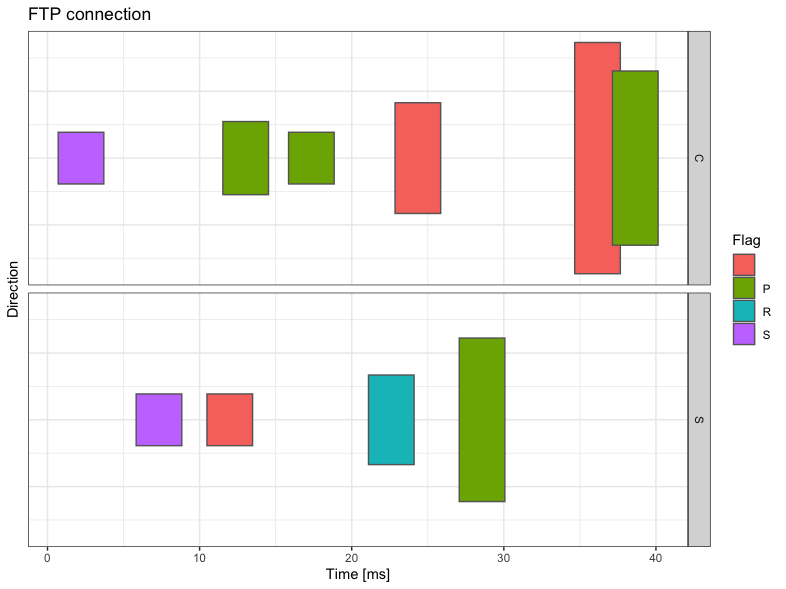
\includegraphics[width=\textwidth]{images/FTP.png}
\caption{Packet sequence in FTP connection}
\end{subfigure}
~
\begin{subfigure}[b]{0.46\textwidth}
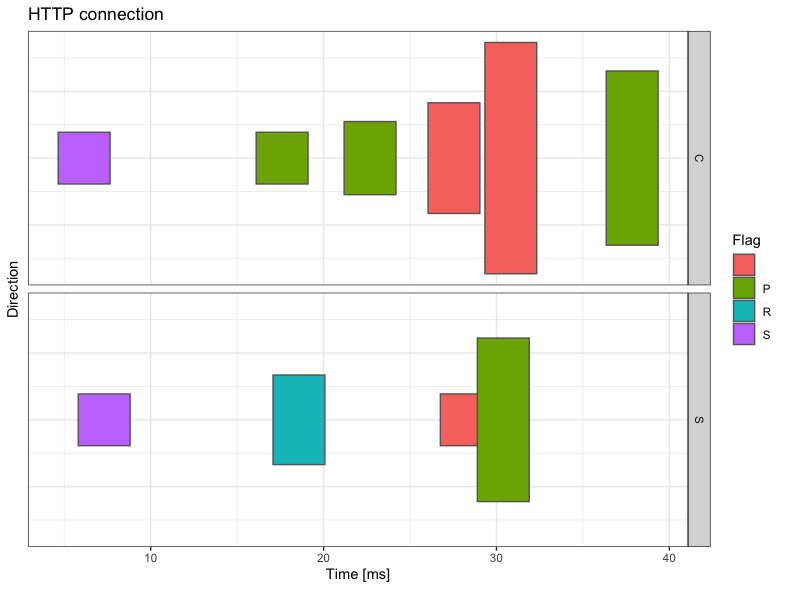
\includegraphics[width=\textwidth]{images/HTTP.png}
\caption{Packet sequence in HTTP connection}
\end{subfigure}
\end{figure}
 
\paragraph{Performed task and application}
The conducted computational task ultimately drives the communication between computers, and thus hugely influences characteristics such as the direction of data transfer, the duration and packet rate, packet sizes as well as the number of connections and performed protocol handshakes to conclude the task. Furthermore, the application used for the task has a significant influence on the generated traffic, as shown for different browser choices by Yen et al. \cite{yen2009browser} or for general application behaviour fingerprinting \cite{stober2013you}. 

\paragraph{Transferred data} 
The amount of transferred data obviously influences the overall packet numbers. Furthermore, the content of the data can potentially impact packet rates and sizes, such as shown by Biernacki \cite{biernacki2017analysis} for streaming services.

\paragraph{Encryption keys}


\paragraph{Caching/Repetition effects}
Tools like cookies, website caching, DNS caching, known hosts in SSH, etc. can cause to parts of a communication being skipped and lead to differences in the captured traffic between initial and subsequent connections.

\paragraph{Captured traffic from background activity} 
In traditional setups, all traffic generated on a host is recorded in the same capture, which makes it hard if not impossible to disentangle traffic from different activities and match them to their origin. Capturing background traffic typically leads to additional flows within the given time interval. $74\%$ of SSH-connections and more than $95\%$ of FTP- and HTTPS-connections in the CICIDS-17 dataset lie within a 5-second interval of connections from other background activity on the same network interface, as depicted in Table \ref{Tab:Sess}.

\begin{table}[h!]
\centering
\begin{tabular}{l|l|l|>{\bfseries}l}
Time&  Source-IP &Destination-IP& Dest. Port\\ \hline
13:45:56.8 & 192.168.10.9 &  192.168.10.50 &       21 \\ \hline
13:45:56.9 & 192.168.10.9 &  192.168.10.50 &    10602\\ \hline
13:45:57.5 & 192.168.10.9 &  69.168.97.166 &      443\\ \hline
13:45:59.1 & 192.168.10.9 &   192.168.10.3 &       53\\ \hline
13:46:00.1 & 192.168.10.9 & 205.174.165.73 &     8080\\ \hline
\end{tabular}
\caption{Exemplary activity interval for host 192.168.10.9 in the CICIDS-17 dataset, containing FTP-, HTTPS- and DNS-, as well as additional unknown activity.}\label{Tab:Sess}
\end{table}

\paragraph{Application layer implementations}
Different implementations for TLS, HTTP, etc. can yield different computational performance and can perform handshakes in slightly different ways. Furthermore, things like multiplexing channel prioritisation can have tremendous impact on the IAT times and the overall duration of the transfer, as shown in a study by Marx et al.  \cite{marx2020same} for the QUIC/HTTP3 protocol.

\begin{figure}
\centering
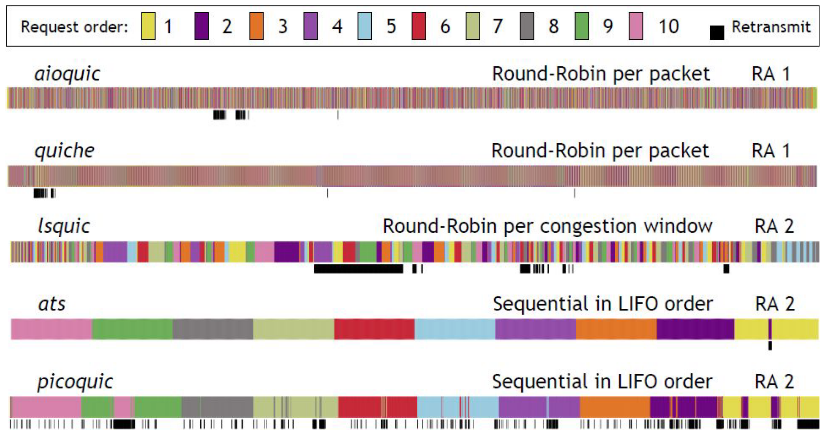
\includegraphics[width=0.8\textwidth]{images/Proto_differences_small.png}
\caption{Comparison of QUIC connection request multiplexing for selected implementations, taken from \cite{marx2020same}}
\end{figure}


\paragraph{Host level load}
In a similar manner, other applications exhibiting significant computational load (CPU, memory, I/O) on the host machine can affect the processing speed of incoming and outgoing traffic, which can again alter IATs and the  overall duration of a connection. \textcolor{red}{Performed various experiments using \textit{stress} under sometimes enormous loads, the startup was a lot slower, but the traffic IATs etc did not change at all, but using Linux bridge and if going via loopback interface in the kernel stack}.

\paragraph{LAN and WAN congestion}
Low available bandwith, long RTTs, or packet loss can have a significant effect on TCP congestion control mechanisms, which in turn influence frame-sizes, IATs, window sizes, and the overall temporal characteristic of the sequence. \textcolor{red}{do we need to verify this? Seems very clear}

\vspace{0.3cm}
Other factors we are currently not considering:

\paragraph{User and scheduled activities}
The frequency with which a user or an application performs tasks governs the larger-scale temporal characteristic of a traffic capture. Since we are focusing on the traffic micro-structures here, we currently omit this impact factor from our analysis. 

\paragraph{Networking stack load}
TCP or IP queue filling of the kernel networking stack can in theory increase packet waiting times and therefore IATs of the traffic trace. However, we did not find any significant effect on the described traffic similarity measures for various amounts of load generated with iPerf, both for regular settings and our design.

%\textcolor{red}{We should perform an experiment using iperf, once with TCP and once with UDP to quantify the effect}.


\paragraph{TCP congestion management implementation}
Different versions of the TCP congestion manager exist on Windows and Linux such as TCP Reno/Tahoe, which can have minor influence on the traffic, as shown by Grieco et al. \cite{grieco2004performance}. Existing implementations on a machine stay mostly constant, which is why we also omit this variable at the moment.
 Implementations within a machine should stay constant.

\paragraph{Network configurations}
Network settings such as the MTU or the enabling of TCP Segment Reassembly Offloading have effects on the captured packet sizes, but like TCP implementations stay mostly constant for a host. 








%\section{Influence factors on traffic characteristics}
%
%\subsection{}
%
%
%\begin{table}
%\begin{tabular}{p{2.5cm}|p{3cm}|p{8cm}}
%Influence& Level & Description \\ \hline \hline
%
%Higher level influence&
%User and scheduled activities&
%How often the user accesses which services, or how often and when a system updates information\\ \hline 
%
%
%Major influence&
%Application used&
%This governs what application layer protocols are used, how often and in what order. As an example, despite doing the same thing, Chrome and Firefox send HTTP-Get requests in different orders and open different numbers of connection sockets\\ \hline
%
%Minor influence&
%Transferred data&
%The size of the transferred data influences overall packet numbers, and potentially the packet rates and sizes (for example streaming high-quality vs low quality), as can the data type.\\ \hline
%
%Major influence&
%Application memory&
%Applications often cache content, credentials, DNS records or cookies from previously contacted hosts\\ \hline
%
%Biggest influence& 
%Application layer protocols &
%Different application layer protocols obviously follow different communication protocols, send data differently, and trigger additional connections in different ways\\ \hline
%
%
%Minor/major influence&
%Application layer implementations&
%Different implementations for TLS, HTTP, etc. can have differing performance, which influences packet IATs and potentially TCP buffering. They can furthermore often differ in minor ways such as different handshakes etc., and occasionally in major ways such as HTTP multiplexing implementations which differ wildly in the channel prioritisation\\ \hline
%
%
%Potential minor influence& 
%TCP implementation&
%There are different implementations of TCP on Windows and Linux such as TCP Reno/Tahoe, which can have minor influence on the traffic but they should stay the same on a machine\\ \hline
%
%Minor influence&
%Network interface load&
%TCP buffer filling due to other programms communicating (both in forward and receiving direction). Potentially other buffers or similar in the networking stack, and therefore the overall bandwidth available\\ \hline
%
%Minor influence&
%Host level load& \\ \hline
%
%Major influence&
%LAN and WAN & Congestion, low bandwith, or loss can have a significant effect on TCP (and others like QUIC) congestion control mechanisms, which in turn influence frame-sizes, IATs, window sizes, ....
% \\ \hline
%
%Minor influence&
%Network configuration&MTU, MTU path discovery, and TCP Segment Reassembly Offloading \\ \hline
%
%\end{tabular}
%\caption{Influence factors}\label{Tab:Influence}
%\end{table}
%Influence factors due to Linux bridge implementation??? Can't find anything on that


\section{DetGen Architecture}

DetGen is a container-based emulator that we developed to enable repeatable, realistic, and flexible network experiments. DetGen extends the widely-used Mininet testbed \textcolor{red}{insert citation} by adding scenarios for benign and attack traffic generation, event labelling, and p

%\section{Background}\label{Sec:b8ackground}

\subsection{Design overview}

The Detgen framework uses Mininet to create a network with a \textcolor{red}{desired} topology, along with virtual software switches, Ethernet links, routers, and firewalls. The network is then populated with containers ,which perform a variety of activities for traffic generation. The conducted activities are composed of scripted \textit{scenarios} (\textcolor{red}{give examples here}), but subject to a high degree of randomisation. The captured traffic events are labelled individually after the specific generating action. 

\subsection{Containerization}
%\textcolor{red}{to do:need to improve}
Containers are standalone packages that contain an application along with all necessary dependencies using OS-level virtualization. In contrast with standard Virtual machines (VMs), containers forego a hypervisor and the shared resources are instead kernel artifacts that can be shared simultaneously across several containers, leading to minimal CPU, memory, and networking overhead \cite{kolyshkin2006virtualization}.


%\textcolor{red}{Although this prevents the host environment from running different operating systems, containerization incurs minimal CPU, memory, and networking overhead whilst maintaining a great deal of isolation} \cite{kolyshkin2006virtualization}. 

Due to the separation of processes, containers provide significantly more isolation of programs from external effects than regular OS-level execution. This isolation enables us to monitor processes better and create more accurate links between traffic events and individual activities than on a virtual machine were multiple processes run in parallel, which can all generate traffic. The one-to-one correlation between containers and network traces allows us to produce labelled datasets with fully granular ground truths. 

Containers are specified in an image-layer, which is unaffected during the container execution.
This allows containers to be run repeatedly whilst always starting from an identical state. In combination with the container isolation, this allows us to perform network experiments that can be easily reproduced by anyone on any plattform \textcolor{red}{insert citation}. 


The container network interface provides the connection between a network namespace and the container runtimes. We want to \textcolor{red}{highlight} that multiple containers can share on network interface, which enables us to generate traffic from multiple applications over one network address in order to emulate \textcolor{red}{fully functional network hosts}.
 

\subsection{Scenario scripting}\label{Sec:Scenarios}

We define a \emph{scenario} as a series of Docker containers conducting a specific interaction, whereby all resulting network traffic is captured from each container's perspective. This constructs network datasets with total interaction capture, as described by Shiravi et al. \cite{shiravi2012toward}. Each scenario produces traffic from either a protocol, application or a series thereof. %Both benign and malicious activities are implemented as scenarios. 
Examples may include an FTP interaction, a music streaming application and client, an online login form paired with an SQL database, or a C\&C server communicating with an open backdoor. A full list of currently implemented scenarios can be found in Section \ref{Sec:ExistScen}.
Each scenario is designed to be easily started via a single script and can be repeated indefinitely without further instructions, therefore allowing the generation of large amounts of data.

Our framework is modular, so that individual scenarios are configured, stored, and launched independently. Adding or reconfiguring a scenario has no effect on the remaining framework.

\subsubsection*{Subscenarios} \label{Sec:Subscenarios}

In contrast to scenarios, \textit{subscenarios} provide a finer grain of control over the traffic to be generated, allowing the user to specify the manner in which a scenario should develop. The aim of having multiple subscenarios for each scenario is to explore the full breadth of a protocol or application's possible traffic behavior. For instance, the SSH protocol can be used to access the servers console, to retrieve or send files, or for port forwarding, all of which may or may not be successful. It is therefore appropriate to script multiple subscenarios that cover this range of tasks.

%Subscenarios are specific to particular scenarios and can be specified when launching that scenario.

%The same applies to malicious activity. For instance, it would be naive for an SSH password bruteforcing scenario to always successfully guess a user's password. Instead, we include a second subscenario in which the password bruteforcer fails.

\subsubsection*{Randomization within Subscenarios}\label{Sec:randomsubscen}

Scripting activities that are otherwise conducted by human operators often leads to a loss of random variation that is normally inherent to the activity.
\textcolor{red}{As mentioned in Section \ref{Sec:problems}, the majority of successful FTP transfers in the CIC-IDS 2017 data consist of a client downloading a single text file.} In reality, file sizes, log-in credentials, and many other variables included in an activity are more or less drawn randomly, which naturally influences traffic quantities such as packet sizes or numbers.

We identify variable input parameters within scenarios and their subscenarios and systematically draw them randomly from suitable distributions. Passwords and usernames, for instance, are generated as a random sequence of letters with a length drawn from a Cauchy distribution, before they are passed to the corresponding container. Files to be transmitted are selected at random from a larger set of files, covering different sizes and file names.

\begin{figure}
 \centering 
 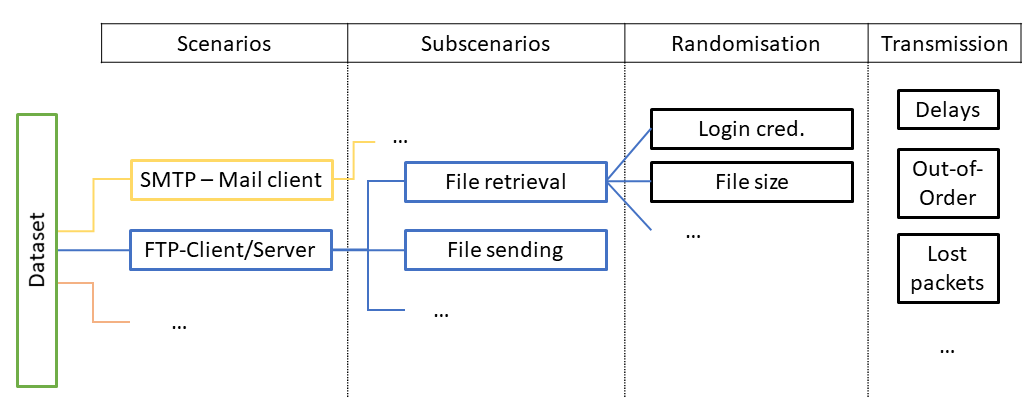
\includegraphics[width=0.780\textwidth]{images/scenario_branching.PNG}
 \caption{Visualization of the different levels at which traffic variation is introduced in DetGen.}
 \label{Fig:branching}
\end{figure}

\subsubsection*{Implementation process}

\subsection{Network creation and population}


To enable communication between containers, we build our framework on top Mininet \textcolor{red}{insert citation} to create virtual networks with customizable topology. 
\textcolor{red}{A topology can be passed to a topology-creation wrapper in matrix form, with diagonal values representing the type of device (switch, container, router, ...), and off-diagonal indicating links}. This allows the import of larger, automatically generated topologies from tools such as \textcolor{red}{insert citation}. 

\textcolor{red}{maybe something about subnets}. 

\subsubsection*{Import of activity timeline}

The modelling and generation of computer network activity has been investigated extensively \textcolor{red}{(citations?)}, and tools to automatically generate realistic network activity streams 

we do not wish to \textcolor{red}{address} this topic here . Instead, our framework imports existing time-series of \textcolor{red}{host flow activity} to generate the corresponding communication. \textcolor{red}{give more info on flow generation tools} 

We transform existing network flow series into an activity timeline by \textcolor{red}{expand this}. We end up with an activity timeline that contains a set of timestamps along with the corresponding scenario and the source and destination host. 

\subsubsection*{Activity conduction}


\subsubsection*{Attack traffic generation}
%\subsubsection{Metasploit and Metasploitable containers}

A description of the capabilities and limitations of both metasploit and the metasploitable VM and the corresponding containers, which we will use.


%\section{Dataset Requirements}\label{Sec:require}

%We can refer to requirements by Cordero et al. (https://arxiv.org/pdf/1905.00304.pdf) on requirements for generating synthetic datasets, and combine them with the existing set of requirements by us. 

%These include:








%In particular, Ring et al. have proposed a method to generate realistic network-wide flow-based traffic that models typical host activity levels. 












%\subsection{Related work and existing datasets}

\subsection{Current data situation}

Currently, intrusion detection researchers predominantly rely on public, synthetically generated datasets, on which NID systems are evaluated subsequently.
\textit{Real-world datasets} such as LANL-15 \cite{kent-2015-cyberdata1} or UGR-16 \cite{macia2018ugr} provide the highest amount of traffic realism, but often lack detailed information such as packet captures due to privacy reasons, and give close to no information on the content of the provided data. 

\textit{Synthetic datasets} such as the CICIDS-17 \cite{sharafaldin2018towards} or the UNSW-16  \cite{moustafa2015unsw} datasets are typically captured in virtual environments that simulate \textcolor{red}{commercial} networks with virtual machines. Traffic is generated from scripted activity, and attack data either injected or generated from carefully inserted vulnerabilities. The arranged settings normally lack the flexibility to generate customized data and by design only provide very limited attack diversity.
%limited insights into the given traffic realism or 

\textit{Attack traffic generators} typically aim at providing traces from a diverse set of attacks, and injecting them into existing traffic captures in various ways. Moirai \textcolor{red}{citation} for example calculates several quantitative characteristics to better embed the attack traffic.  However, most of the issues surrounding real-world traffic captures remain, and there is concern about the realism of injected attack traffic \textcolor{red}{citation}.

Recently, some effort have been made to to generate completely artificial traffic data with \textit{generative adversarial networks} (GANs) trained on real-world traffic. While examples such as DoppelGANger or Ring et al. \textcolor{red}{citation} are successful at generating realistic large-scale network features such as activity levels or \textcolor{red}{connection graphs}, they are not aimed at intrusion detection and do not provide the necessary granularity to model connection- or packet-level features.

 \textit{Testbeds} such as Mininet offer tremendous \textcolor{red}{flexibility}, but are so far not targeted for intrusion detection and lack suitable small-scale traffic generation tools, labelling capabilities, or attack scenarios. 


%A similar description on existing frameworks and datasets as in the existing paper, with a slightly higher focus on existing testbeds and existing container tools.
%\dots \dots
%\dots \dots
%\dots \dots

%\subsubsection{Datasets}
%
%real:
%Los Alamos National Laboratory (LANL)
%University of Granada (UGR)
%
%SANTA
%Only flows, manually labelled
%
%
%CAIDA 2016
%
%MAWI 2000
%
%LITNET
%
%synthetic:
%
%CICIDS-17
%UNSB-16
%
%CIDDS-001
%Python scripts are used for emulating benign user behaviour like browsing the web, sending and receiving emails, as well as exchanging files. To ensure as realistic user behaviour as possible, clients perform their activities with respect to an individual working schedule which considers working hours and lunch breaks.
%
%NGIDS-DS
%Uses IXIA Perfect Storm, also collects host logs
%
%
%
%frameworks:
%
%FLAME
%ID2T
%Use real traffic as input to add attack traffic
%GEN-ESIDS
%HTTP attack traffic after user-based attack description
%NDSec-1 - Also overlaying normal data with attack traffic
%
%Moirai
%
%
%A flow trace generator using graph-based traffic classification techniques
%extractstraffictemplatesfromrealnetworktraf-fic.Then,theirgeneratorusesthesetraffictemplatesinordertocreatenewsyntheticflow-basednetworktraffic
%
%INSECS-DCS
%
%
%
%
%Flow-based network traffic generation using Generative Adversarial Networks
%DoppelGANger
%
%weak:
%PACGAN
%PCAPGAN
%SynGAN
%
%
%surveys:
%A Taxonomy of Network Threats and the Effect of Current Datasets on Intrusion Detection Systems
%
%On the generation of synthetic attacks
%
%
%Docker data generation 
%
%weak on activity generation, only system calls:
%A dataset generator for next generation system call host intrusion detection systems
%Standardized container virtualization approach for collecting host intrusion detection data
%
%
%Notes:
%However, currently available datasets lackreal-life characteristics of recent network traffic. ... IDS is unableto adapt to constant changes in networks (i.e. new nodes,changing traffic loads, changing topology, etc.). Networks areconstantly changing, for this reason depending solely on olddatasets doesn’t help the advancement of IDS(Taxonomy ...)
%
%
%%To evaluate their ability to model the behaviour of a network and to identify malicious activity and network intrusions, new methods have to be tested using existing datasets of network traffic. 
%
%%This network should ideally contain realistic and representative benign network traffic as well as a variety of different network intrusions. 
%
%
%Network traffic contains a vast amount of information about a network and its users which makes it  notoriously difficult to release a comprehensive dataset without infringing the privacy and security rights of the network users \cite{sperotto2009labeled}. In addition, the identification of malicious traffic in network traces is not straightforward and often requires a significant amount of manual labelling work. Currently, only \textcolor{red}{four} intrusion detection datasets exist that contain traffic from real networks, all of which are \textcolor{red}{presented} as anomimised network flows . 
%
%\textcolor{red}{Rework!}The most recent and notable real-world datasets have been released from the Los Alamos National Laboratory (LANL) in 2015 and 2017 \cite{akent-2015-enterprise-data, turcotte17}, and the University of Granada (UGR) in 2016 \cite{macia2018ugr}. Both datasets contain network flow traffic data from a large number of hosts collected over multiple months, giving an accurate representation of medium- to large-scale structures in benign traffic. However, the amount of attack data is small and insufficient for accurate detection rate estimation. Furthermore, packet-level data is not available for both datasets. 
%
%Other real-world datasets, such as CAIDA 2016 \cite{walsworth2015caida} or MAWI 2000 \cite{sony2000traffic}, provide packet headers, but are unstructured and contain no labeled attack data at all.
%
%To improve the lack of attack traffic in NIDS datasets, several artificially created datasets have been proposed. For this, a testbed of virtual machines is usually hosted in an enclosed environment to prevent any malicious code from spreading to other machines on other networks. To generate attack traffic, these machines are then subject to a selection of attack carried out by other machines in the environment. Benign traffic is generated using commercial traffic generators such as the \emph{IXIA PerfectStorm tool}, or by scripting a selection of tasks for each machine. Synthetic datasets cover a smaller timeframe and contain traffic from a small number of hosts. Notable examples are the CIC-IDS 2017 dataset from the Canadian Institute for Cybersecurity \cite{sharafaldin2018towards}, %the CTU-2013 dataset from the \emph{Stratosphere Laboratory} in Prague \cite{noauthor_ctu-13_nodate},
%and the UNSW-NB 2015 dataset from the University of New South Wales \cite{moustafa_unsw-nb15:_2015}. Both datasets contain traffic from a variety of attacks, and are available as packet headers or as network flows with additional features crafted for machine-learning. While the benign traffic for the CIC-IDS 2017 data was generated using scripted tasks from a number of host profiles, the benign data for the UNSW-NB 2015 data is a mixture of captured real traffic from another subnet and traffic generated using a commercial traffic replicator. 
%
%
%%We omitted the synthetic KDD-Cup 1999 and the DARPA 1998 datasets along with their derivates from the discussion as they are well-known to be outdated and contain unrealistic benign traffic, artificially high benign/attack data ratios, and artifacts stemming from communication simulations \cite{tavallaee2009detailed,mchugh2000testing}, problems which have been addressed by most modern datasets.
%
%Container networks have recently been adopted to conduct traffic generation experiments, such by Fujdiak et al. \cite{fujdiak2018ip} who use containerized web servers to collect DoS-traffic. Furthermore, significant effort has been put into the creation of large-scale virtualization frameworks to provide automatized network testbeds \cite{crussell2015minimega, badiger2018violet}.
%
%


%\subsubsection{Problems in modern datasets}\label{Sec:problems}
%
%We can import here a lot from the existing paper, but add the following issues:
%\begin{enumerate}
%\item Invalid/Inconsistent traffic
%\item Extensibility of the attacks
%\item Lack of open-source implementation of attack traffic generation, which makes difficult to understand what exactly was detected
%\item Lack of related data sources
%\end{enumerate}


%\subsection{Containerization with Docker and Mininet}
%%\textcolor{red}{to do:need to improve
%
%A similar description on Containers and Docker as before, extended by a description of Mininet
%\dots \dots
%
%\dots \dots
%
%\dots \dots



%\subsection{Dataset Requirements and benefits of our framework}
%
%Here, we can point to a set of requirements by Cordero et al. (https://arxiv.org/pdf/1905.00304.pdf) for generating synthetic datasets.
%%This should potentially be merged with the dataset requirements, I am currently unsure where to put this. 
%
%\section{Design}\label{Sec:Design}
%
%Explain the general idea and benefit of using containers for traffic generation in comparison to regular testbeds, similar to the existing paper.
%
%\dots \dots
%
%\dots \dots
%
%\dots \dots
%\subsection{Modes of Operation}
%
%\begin{enumerate}
%\item Stand-alone scenarios for traffic generation
%\begin{itemize}
%\item Straightforward generation of traffic for the selected service
%\item Easy to costumize and can be used as prior testing for modifying services in the other two options
%\end{itemize}
%\item Network-wide activity emulation
%\begin{itemize}
%\item A topology is generated randomly with a set of hosts and corresponding services running on them
%\item Scenarios are started and hooked to corresponding host network interfaces according to a launch script that emulates empirical activity measurements
%\item These activity measurements come in the form of a timeline of events that can be drawn from a set of basic distributions that we provide or can be generated by third party such as the GAN in the Doppelganger paper (this way we can avoid being scrutinised for a lack of realism in this field).
%\end{itemize}
%
%
%\item Microservice activity emulation
%\begin{itemize}
%\item In this mode, we set up a VM that hosts a number of service containers and emulates the situation of a typical microservice host
%\item We run the same scenarios, but the client containers are located on another machine. 
%\item We collect system call logs from both the containers and the host
%\item This is the least developed mode, but the additionally collected system calls give the most realistic picture in this state
%\item It might be good to define and describe this setting already if we want to implement any container-specific attacks and models in the future
%\end{itemize}
%
%\end{enumerate}
%
%
%
%
%
%\subsection{Scenarios and subscenarios}
%\label{Sec:Scenarios}
%Here we describe the design process of the scenarios, just like in the previous paper.
%
%\subsubsection{Randomization}\label{Sec:randomsubscen}
%\dots \dots
%
%\dots \dots
%
%\dots \dots
%\subsubsection{Network transmission}\label{Sec:Netrand}
%\dots \dots
%
%\dots \dots
%
%\dots \dots
%
%\subsubsection{Implementation Process}
%\dots \dots
%
%\dots \dots
%
%\dots \dots
%
%\subsubsection{Attack generation with Metasploit/Metasploitable}
%\dots \dots
%
%\dots \dots
%
%\dots \dots
% 
%%\subsection{Implemented scenarios}\label{Sec:ExistScen}
%
%
%%\begin{figure}%[h!]
%%\centering
%%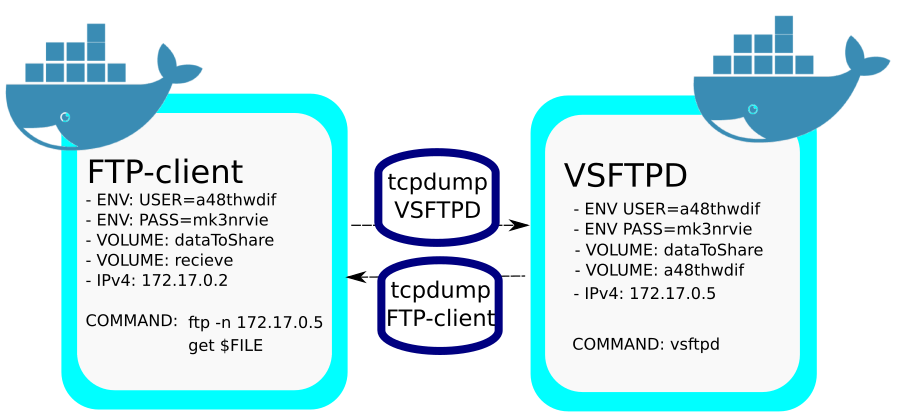
\includegraphics[width=0.49\textwidth]{images/ftp_new1.png}
%%\caption{Diagram of FTP scenario}
%%\end{figure}
%
%
%\subsection{Network-emulation}
%
%Describe the design of how the topology is generated before the data capture is started, and how the scenarios are launched and stopped during the data capture.
%\subsubsection{Topology generation}
%\dots \dots
%
%\dots \dots
%
%\dots \dots
%\subsubsection{Launch-script}
%
%\dots \dots
%
%\dots \dots
%
%\dots \dots
%
%\subsubsection{Dataset coalescence}\label{Sec:datasetcreation}
%\dots \dots
%
%\dots \dots
%
%\dots \dots
%\subsubsection{Activity timeline input}
%Here, we describe how the activity timeline in the launch script can come from unsophisticated distributions that we include, or from sophisticated 3rd party models such as Doppelganger. Since the modelling of computer activity is a field of ongoing research, it seems best to shift the responsibility for realistic models away by allowing this input. 
%
%\subsection{Microservice-emulation mode}
%
%\dots \dots
%
%\dots \dots
%
%\dots \dots


\section{Fidelity confirmation experiments}\label{Sec:Experiments}

This section is important to demonstrate that our data is valid and overcomes the difficulties entailed with synthetic data generation. Cordero et al. have proposed some more simple test that we can refer to first

\textcolor{red}{Question to be answered}: What requirements are there for the additional data, program logs and system logs, that we collect? Should we put less emphasise on these data sources in general if we are not able to perform these tests, and refer to them in future work? I am not aware of any papers that discuss these requirements in a similar way. 



\subsection{Traffic similarity metrics for determinism and realism evaluation}

We now assess the claim of control over the outlined traffic influence factors, and how similar traffic generated with the same settings looks like. We also demonstrate that this level of control is not achievable on regular VM-based NIDS-traffic-generation setup.
To do so, we require a similarity metric that measures how similar or dissimilar two traffic traces are. We want to compare traffic similarity on three ...

we compare our framework against a setup on a virtual machine to show that we provide deterministic control that is not achievable on a common setup. For that, we measure traffic similarity using a set of similarity metrics on traffic both from our and the comparison setup. The traffic is subject to varying degrees of influence from the above described impact factors. We show that when all factors are held constant, our traffic is much more similar than on a regular setup.

%We should also demonstrate how difficult it is to match all flow events to specific events (I am still unsure how), and how often you get system background events (very straightforward using flow counting and port entropy).

%Common setup: Network of VMs with each VM representing one host in a regular network. Multiple services with scheduled scripted activities running on a VM. Traffic captured at router or network interface. 

\begin{itemize}
\item \textbf{Overall connection similarity} We collect 80 flow summary statistics (IAT and packet size, TCP window sizes, flag occurrences, burst and idle periods). We compress this information using PCA to 8 significant dimensions, and measure the cosine similarity between connections, which is also used in general traffic classification \cite{aun2017review}.
\item \textbf{Flow level similarity} To quantify the similarity of flow sequences, we assign each flow a discrete state, according to its port, size quantile, and interarrival time quantile. We then calculate for a group of captures the probabilities of flow states at each step in the sequence, and use the average sequence likelihoods of each group as a similarity measure. 
\item \textbf{Sequential similarity} To quantify the similarity of packet sequences in traffic captures, we proceed in a similar fashion and assign packets a discrete state according to their flags, direction, sizes, and interarrival times. We then calculate the Markovian probability of each packet state conditional on the previous packet. We do this for sequences of 15 packets at the start, the middle, and the end of a connection, and use the average sequence likelihood of each group as a similarity measure. If connections are completely similar, the conditional probabilities and thus the likelihoods should converge to one.
\end{itemize}

In contrast to 


\subsubsection{Constant settings}

We now apply the described similarity measures to different groups of traffic traces to evaluate the \textcolor{red}{determinism} of our data generation process. We vary the control settings of the described influence factors, described in Section \ref{Sec:Impactfactors}, for each group, but keep them constant within each group. We use three different traffic types (HTTP, file-syncing (port 8384), and botnet), for which we both perform different application-specific activities and create different overall settings. We furthermore perform the same HTTP-activities on two regular VMs without containerisation, but with the same settings.


\begin{table}
\centering
\begin{tabular}{p{1cm}|p{3cm}|p{3cm}|p{3cm}|p{2cm}}
Label &Overall Setting&HTTP&File-Sync & Mirai-C\&C\\ \hline
A&\textcolor{red}{Little congestion, high comp. load} & Get-request on NGINX/wget, small file & Sequence 1,  syncing to two computers & Command sequence 1 \\ \hline
B& Moderate congestion, low comp. load &Multi-request for different fixed files, NGINX & Sequence 2,  syncing to four computers & Command sequence 2\\ \hline
C& High congestion, no comp. load & Post-request on Apache/wget, large file &Sequence 3,  syncing to two computers & Command sequence 3\\ \hline
D& High congestion, high comp. load & Multi-request for different fixed files with caching, Apache & Sequence 4,  syncing to four computers & Command sequence 4\\ \hline

\end{tabular}
\caption{Test}\label{Dataset}
\end{table}

\begin{figure}
\centering
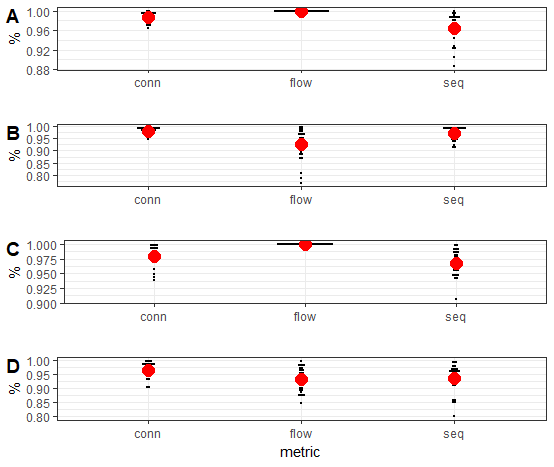
\includegraphics[width=.9\textwidth]{images/Determ-metric.png}
\caption{HTTP}\label{determ-metric}
\end{figure}


\subsubsection{First test: Determinism}



\subsubsection{Second test: Realistic diversity under all impact factors}


Here, we apply the simulation of all impact factors simultaneously to our traffic and test if the traffic similarity scores are as divergent as for traffic from a real-world dataset (i.e. CAIDA) for two or three exemplary protocols, and we also compare it to the same protocols in the CICIDS-17 dataset. This will let us argue that we can achieve realistic levels of diversity (something criticised by Sommer-Paxson), and that our framework lets researchers explore higher levels of diversity than currents labelled solutions.




%\subsection{Data correctness tests}

%This section is concerned with dataset defects, artifacts, or invalid data (inconsistent MTU etc.). These are very straightforward to test and should not take up much space. 


%\subsection{Diversity tests}

%These tests, also from Cordero et al. quantify diversity via the entropy of different quantities such as IP diversity, Time-to-Live, Maximum-segment-size, Window size, ToS. I think we should keep this relatively short and omit comparison to other datasets since this is already done by Cordero et al. 


%\subsection{Structural dataset dimensionality}



%Autoencoders are often used to compress non-deterministic, noisy data. Bahadur et al. have developed a procedure to estimate the ,,dimensionality'' (to be understood as the complexity) of a dataset using variational autoencoders. I believe we can transfer this concept to sequence compression and estimate the overall complexity of connection sequences in our framework with both real traffic captures and existing network intrusion datasets. 

%Showing that our data is closer to real-world data would be a good test for "artificially predictable patterns", as described by Cordero et al., and go hand-in-hand with demonstrating the benefits of our framework for the training of deep-learning models. The importance of data that is less artificially predictable and closer to real-life traffic in terms of statistical variations lies in its suitability as a benchmark for detection rates, since less complex data is easier to train on and yields unrealistically high detection rates. 


%Measure structural richness of
%Also measure divergence across same activities (same activity and same port)
%Demonstrate benefit of structural richness
%Closer to reality



%\subsection{Reproducible scenarios}\label{Sec:deterministic}

%\dots \dots

%\dots \dots

%\dots \dots
%\begin{figure}
%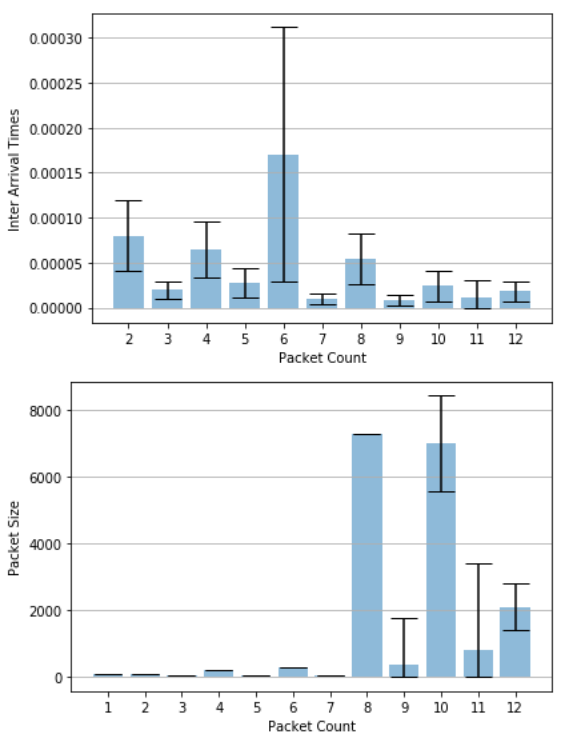
\includegraphics[width=0.45\textwidth]{images/combined3.png} % first figure itself
%\caption{Means of IATs \& packet sizes along with standard deviation bars for the first twelve packets in the Apache scenario.}
%\label{fig:size1}
%\end{figure}

 


% Need to edit these sections to provide a single context for both the artificial delays & classification

\subsection{Explorating Artificial Delays}

This section is already existing, we could potentially expand this. I think it is sufficient and analysing it more does not add much to the paper as the performance of TC netem is relatively well accepted. I think we could even move this section to the appendix.

%\begin{figure}
%\captionsetup{justification=centering}
%\centering
%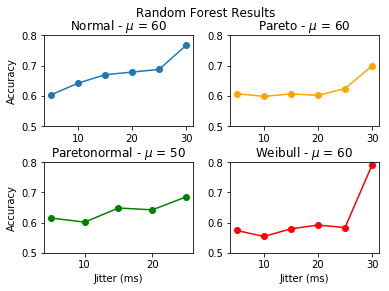
\includegraphics[width=0.45\textwidth]{images/1-plot_exp1.png}
%\caption{Results of Random Forest Classifier for a given distribution at the best performing delay mean $\mu$. Note that a score of .5 indicates total indistinguishability.}
%\label{Fig:rf_graph}
%\end{figure}
%
%
%
%\begin{table}[ht!]
%\begin{center}
%\begin{small}
%\begin{sc}
%\begin{tabular}{ccccc}
%\hline
%Distribution & Mean & Jitter & RF Accuracy\\
%\hline
%No Delays (Baseline) & 0 & 0ms & 0.8176 \\
%Constant Delay & 40ms & 0ms & 0.6730 \\
%Normal & 60ms & 5ms & 0.6028 \\
%Pareto & 60ms & 10ms & 0.5979 \\
%Paretonormal & 50ms & 10ms & 0.6015 \\
%Weibull & 60ms & 10ms & 0.5540 \\
%\hline
%\end{tabular}
%\end{sc}
%\end{small}
%\caption{Worst Random Forest accuracy rates for a given distribution}
%\label{tab:results-iat_rf}
%\end{center}
%\vskip -4mm
%\end{table}



\section{Use-cases}


\subsection{Benefits of ground-truth labels}
Possible title: \textbf{Exploring the effect of rare events to model performance}

Extensive ground-truth labels for our activities are arguably the most important contribution of the DetGen framework, so we should highlight their benefit most. Since ground-truth labels on attack data are existing in other datasets, we should emphasise the benefit of having labels for different activities. In my eyes, the most striking benefit arises for false-positive analysis, which we could then combine with showcasing the benefit of being able to generate different amounts of traffic for different activities.


\paragraph{Plan}
Implement the LSTM-model in the paper "An LSTM-Based Deep Learning Approach forClassifying Malicious Traffic at the Packet Level", train it on our data (both benign and attack traffic). Extract labels of traffic responsible for false-positives, show how much they are clustered around particular activities (potentially rare activities) compared to the overall traffic. Give potential reason for this. Generate a new dataset with increased amounts of the activities responsible for false positivies. Demonstrate that false-positives decrease.

%\subsubsection{Benefits of structural richness}
%
%Possible title: \textbf{Harder benchmarks}
%
%As described above, the importance of data that is less artificially predictable and closer to real-life traffic in terms of statistical variations lies in its suitability as a benchmark for detection rates. In particular, we want to demonstrate that our data functions is a more difficult and realistic benchmark that is less prone to inflating detection rates than existing datasets, something that is often a point of criticism for models evaluated on synthetic data. 
%
%To show that the training and detection is harder on our data, we could generate a dataset with similar attacks and services as the CICIDS-17 dataset, and train the above described LSTM model on both datasets. We could show that the training loss goes down more slowly on our data, as well as other metrics (increased validation loss --> overfitting etc.). We could then go ahead and show that the same attacks are detected easier by the same model in the CICIDS-17 data than in our data, concluding that it is a less realistic benchmark.
%
%It would be good to also include a comparison with actual real-world traffic here to bolster our conclusion, but due to the lack of structured real-life datasets it is difficult to create a fair and scientific comparison. 
%
%%\subsubsection{Show utility of tuning amount of rare events}
%
%\subsection{Show utility of flexible topology}
%
%This is another possibility to demonstrate that the flexibility provided through containerisation allows for better benchmarking and more in-depth evaluation.
%
%Methods aiming at modelling network structures are an established method for botnet and pivoting detection. Even though the network topology is a crucial variable in their training, their evaluation is to my knowledge only done on single static datasets such as the LANL-15. 
%
%My idea is that we generate about 10 datasets with different topologies, (especially different numbers of subnets and servers), and highlight the variation in prediction accuracy, i.e. the accuracy on one dataset is significantly higher/lower, and the average across the different datasets is a better indicator that eliminates the topology as a variable. We do not necessarily need to implement any attack traffic here since the modelling accuracy on benign traffic should be sufficiently quantifiable. 
%
%A suitable candidate for the evaluation would be the paper "Link prediction in dynamic networks using randomdot product graphs", which comes from people at Imperial College that I know. The model tries to give a probability for each connection to appear in a network, in order to spot connections between unlikely pairs as anomalous behaviour. I could ask the people for the implemented model so we do not have to do it ourselves, or we could even have a chat with them.
%
%
%%\begin{figure}%[ht!]
%%\subfloat{%
%% 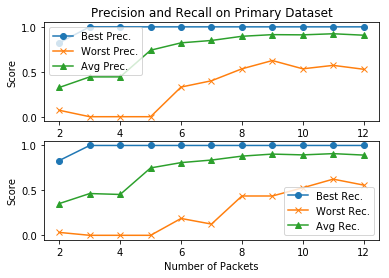
\includegraphics[width=0.4\textwidth]{images/bw_100_exp_3.png}}
%%\subfloat{
%% 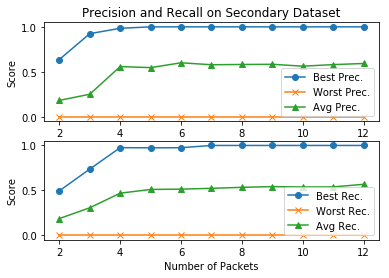
\includegraphics[width=0.4\textwidth]{images/bw_500_exp_3.png}}
%%\caption{Results of Random Forest Classification on Primary dataset (Above) and Secondary dataset (Below)}
%%\label{Fig:Primary}
%%\end{figure}
%
%\subsection{Customisable attack traffic by using metasploitable}
%
%Rob and I discussed that by using a combination of a metasploit-attack container and a metasploitable-victim container, we could generate and embed a significantly larger number of attack traffic types more efficiently than we are currently. Since we can attach the metasploitable-container to the network interface of regular containers, we can embed the implemented vulnerabilities very easily in a given scenario. Furthermore, since both containers are well maintained, we can keep the attack catalogue up-to-date.
%
%I think the best use-case is to showcase the process of adding a new type of attack to the dataset, embedding it in a proper way to a given scenario, generating data from it. We could additionally implement a corresponding detection method, but I think this would not demonstrate anything. 
%
%
%\subsection{Simple use-case for the microservice mode?}
%This use-case depends a lot on the state of the framework, but we could in principle show the benefits of the framework for the recently published model in "AppMine: Behavioral Analytics for Web Application Vulnerability Detection" on a more extensive dataset, since they only had very limited data available. 
%\section{Conclusions}\label{Sec:Conclusion}
%
%
%
%\subsection{Difficulties and limitations}


\subsection{Future work}



%Syslog logging driver
%add server to capture syslogs 

%https://docs.docker.com/config/containers/logging/syslog/


%We are grateful for our ongoing collaboration with our industry partners  on this topic area, who provided both ongoing support and guidance to this work. Discussions with them have helped reinforce the need for a better evaluation and understanding of the possibilities that new intelligent tools can provide.

%Full funding sources after currently blinded.

\bibliographystyle{abbrv}
 
\bibliography{DetGen_ext}

%\appendix


\end{document}
